\documentclass[12pt]{article}
\usepackage[margin=0.8in]{geometry}
\usepackage{amsmath}
\usepackage{hyperref}
\usepackage{graphicx}
\usepackage{float}
\usepackage{caption}
\usepackage{subcaption}
\usepackage{listings}

\title{Numerical analysis: Assignment 8}
\author{Niccolo Zuppichini}
\begin{document}

\maketitle
\section*{Exercise 1}


\begin{equation}
	x^* = \textrm{arg min}_{x \in \mathcal{R}^n} ||b - Ax||
	\label{eq:initial}
\end{equation}


A solution to Equation \ref{eq:initial} is also a solution to: \\

\begin{equation}
	\frac{\partial}{\partial x} ||b - Ax||
\end{equation}

By expanding the norm and taking the derivative and setting it to zero:

\begin{equation}
	\begin{split}
		\frac{\partial}{\partial x} ||b - Ax|| = \frac{\partial}{\partial x}  <b - Ax, b - Ax> = \\
		= \frac{\partial}{\partial x} (b - Ax)^2 = \frac{\partial}{\partial x} b^2 + (Ax)^2 - 2 b^T Ax = 2 A^T A x - 2 A^T b = 0  \\
		\implies  A^T A x = A^T b
	\end{split} 	
\end{equation}

Which is the normal equation. \\

\section*{Exercise 2}

The code has been implemented in \textit{exercise2.py}. The output of my code is reported in Lst. \ref{lst:output} and in Fig. \ref{fig:output} : \\

\begin{lstlisting}[caption=Code output, label=lst:output]
To reach an error of 1e-07 it took 255 iterations
Optimal parameter values :  [45.20164   19.809147  -5.4695835 69.520905 ]
Model parameters:  [-2.86684774 -4.09136652  5.33633989]
\end{lstlisting}

\begin{figure}[h]
\centering
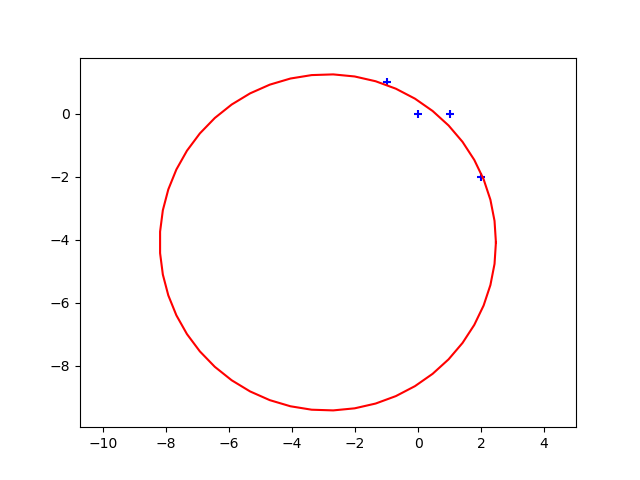
\includegraphics[width = 0.7 \linewidth]{ex2plot.png}
\caption{Result parametric circle model F}
\label{fig:output}
\end{figure}


\end{document}